\section{Testing}
I am going to hand compile and trace a series of programs to validate that the system is functioning correctly, as well as demonistrating various error messages the compiler can produce should it encounter syntax errors within the source code. I will also demonstrate how the graphical display and debugger for the virtual machine work - showing the robustness and performance of the system by compiling and executing a game of pong. Below is the link to the testing video:

https://www.youtube.com/watch?v=KQ6ibE77F8w

\subsection{Testing Table}

\begin{longtable}{|p{1cm}|p{5cm}|p{5cm}|p{2cm}|} 
    \hline
        No & Test & Purpose & Timestamp \\ 
    \hline
        1.1
        & 
        Assemble a program that counts to 15. 
        &
        To ensure the assembler correctly assembles programs into machine code.
        & 
        10:53-14:30
        \\
    \hline
        1.2
        & 
        Assemble a program containing branch and jump instructions between labels.
        &
        To ensure jump instructions calculate absolute addresses, and branch instructions calculate relative offsets. Validates that the assembler can correctly use the position of labels within the source code to determine these values.
        & 
        14:30-16:26
        \\
    \hline
        1.3
        & 
        Assemble a program containing macro instructions.
        &
        To ensure that the assembler can correctly expand and assemble macro instructions by validating the number of instructions produced and their opcodes.
        & 
        16:26-18:33
        \\
    \hline
        1.4
        & 
        Attempt to assemble a program containing an invalid character.
        &
        To ensure the assembler halts compilation and throws a syntax error, pointing out the position of the invalid character in source code.
        & 
        18:47-19:12
        \\
    \hline
        1.5
        & 
        Attempt to assemble a program containing a undefined mnuemonic.
        &
        To ensure the assembler halts compilation and throws a syntax error, specifying that the mneumonic encountered is not defined within the instruction set.
        & 
        19:18-19:30
        \\
    \hline
        1.6
        & 
        Attempt to assemble a program containing an overflowinging integer.
        &
        To ensure the assembler throws an error specifying that the number it is attempting to assemble is too large to fit in 16 bits. 
        & 
        19:30-19:40
        \\
    \hline
        1.7
        & 
        Attempt to assemble a program containing an unexpected register or invalid label.
        &
        To ensure the assembler throws an error specifying that the label hasn't been defined within the program, or that the register doesn't exist. 
        & 
        19:40-20:15
        \\
    \hline
        2.1
        & 
        Trace the execution of a program to count to 15.
        &
        Ensure the computer exhibits the correct state and control flow when executing a binary executable. 
        & 
        21:10-22:20
        \\
    \hline
        2.2
        & 
        Trace the execution of a program containing jump and branch instructions.
        &
        Validates whether the virtual machine can correctly jump between instructions and follow the control flow specified within the program.
        & 
        22:20-24:14
        \\
    \hline
        2.3
        & 
        Trace the execution of a program to calculate the factorial of a number.
        &
        An integration test for the assembler and virtual machine together in order to assemble and execute a more complex program involving the stack and subroutines. 
        & 
        24:15-26:47
        \\
    \hline
        2.4
        & 
        Test the graphical display by executing programs that involve writing piexls to the screen.
        &
        Ensures the state of pixels on the screen directly correspond to the state of VRAM. Validates that writing to the screen via offsets, and within a loop function as expected.
        & 
        26:47-30:35
        \\
    \hline
        3.1
        & 
        Write and compile a program in the high level langauge to calculate the factorial of a number.
        & 
        Demonstrate that the assembly code produced, after being copiled and executed - correctly exhibits the functionality of the high level program.
        & 
        31:50-34:17
        \\
    \hline
        3.2
        & 
        Attempt to compile a program containing an unexpected keyword.
        &
        Validate that the compiler halts compilation and throws a syntax error pointing out the location of the error, and suggesting alternative keywords to fix the issue. 
        & 
        32:15-32:35
        \\
    \hline
        3.3
        & 
        Attempt to compile a program without a main subroutine
        &
        Validate that the linker throws an error when attempting to compile a program without an entry point. 
        & 
        32:30-32:38
        \\
    \hline
        3.4
        & 
        Attempt to compile a program attempting to assign a value of the incorrect type to a variable.
        &
        Ensure that the compiler throws a type error and halts compilation. 
        & 
        32:50-32:58
        \\
    \hline
        3.5
        & 
        Compile and execute a program that uses VRAM and the graphical display to demonstrate passing by value and reference within my language. 
        &
        Demonstrate how dereferencing pointers to variables can be used within a subroutine to modify 'external' variables, and how to write to memory by dereferencing a memory location including using pointer aithmetic for offsets. 
        & 
        34:22-36:36
        \\
    \hline
        3.6
        & 
        Attempt to compile a program containing a reference to an undeclared subroutine.
        &
        Ensure that the compiler halts compilation and points to the location of the undeclared subroutine in the source code.
        & 
        36:36-36:47
        \\
    \hline
        3.7
        & 
        Compile and exeute a program that demonstrates pointer arithmetic. 
        &   
        Validates pointer arithmetic, dereferencing and memory addresses all function correclty within the langauge. Including that dereferencing a variable declared as a pointer to another variable, who's since had its contents changed - should, when dereferenced - also exhibit that new value. 
        & 
        36:48-38:48
        \\
    \hline
        3.8
        & 
        Compile and exeute pong. 
        &   
        An integration test that demonstrates how all three components of the system can function together to compile a complex program that involves all elements of the langauge: subroutines, stack frames, constants, conditionals and loops, pointers and references, etc. And furthermore how the CPU can use a delay timer to create a game playable in real time that interfaces with a keyboard. Ensuring the system is sufficiently optimised to execute at 60 frames per second. 
        & 
        38:38-41:50
        \\
    \hline
\end{longtable} 

\subsection{Testing Key Algorithms}

\subsubsection{Parsing}
The first part of the system I want to test in more detail is the parser. I will run a series of tests that ensure each type of program statement is successfully parsed into the desired nodes, and the system throws the required errors when it encounters invalid syntax.

\begin{longtable}{|p{12cm}|p{4cm}|} 
    \hline
        Program & Result \\ 
    \hline
        \raisebox{-\totalheight}{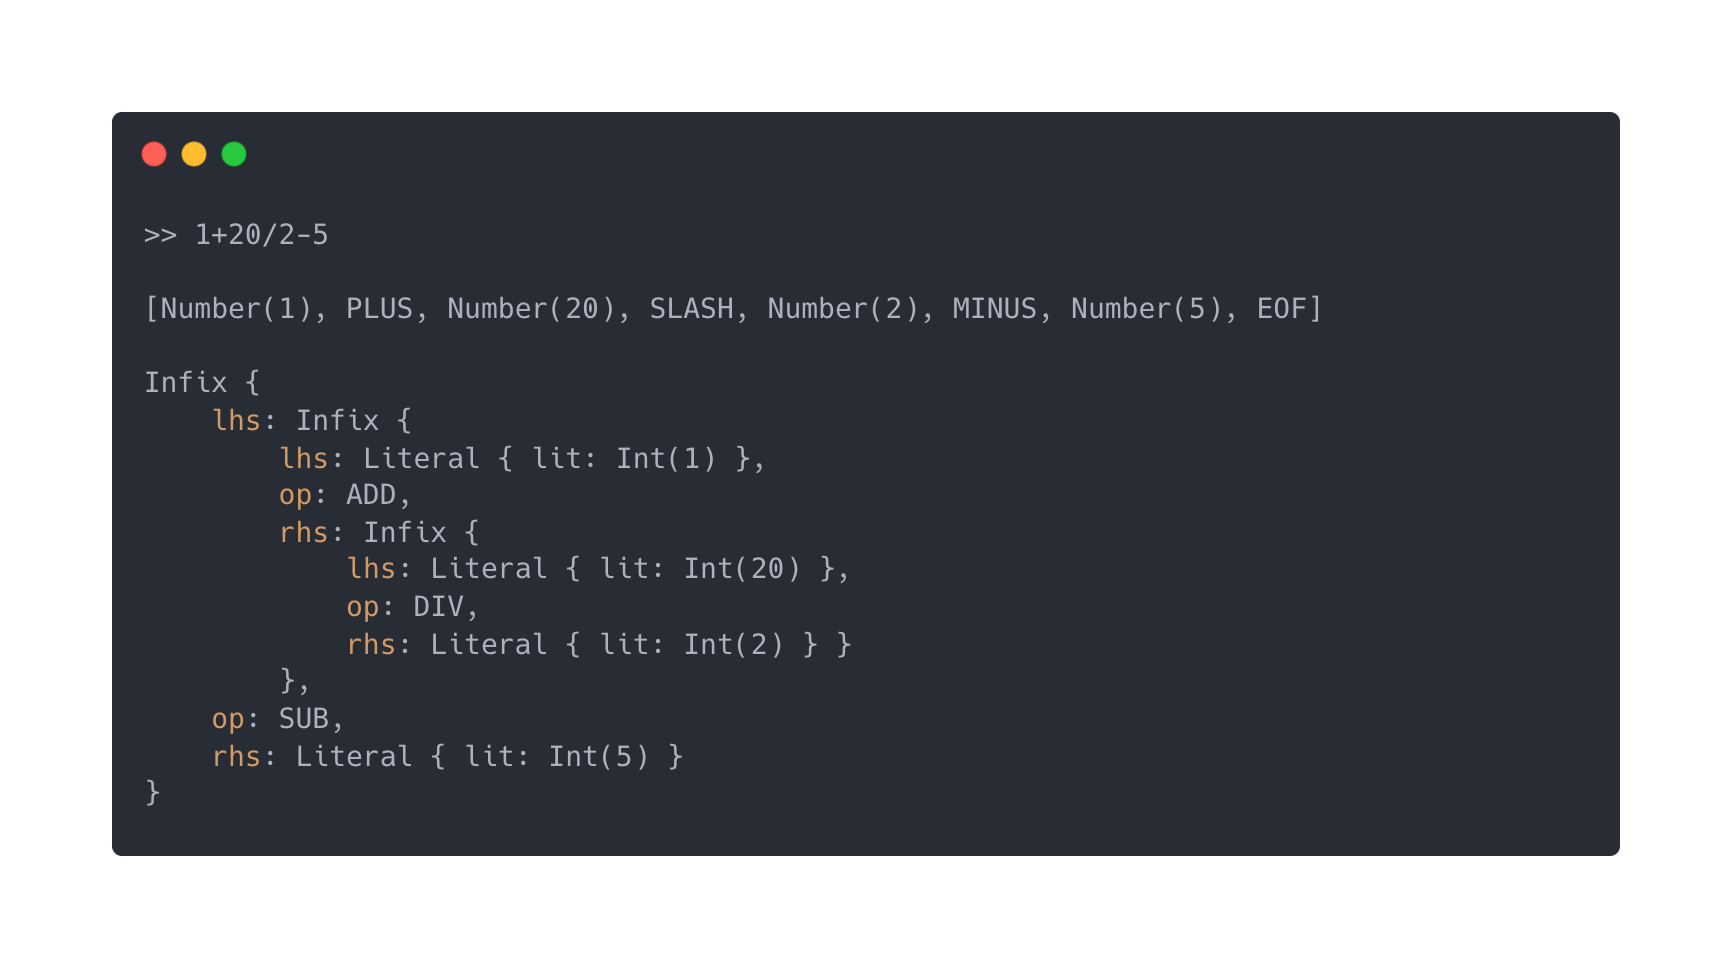
\includegraphics[width=12cm]{1. Unit Test.png}}
        & 
        The correct tokens and AST have been produced, matching the initial expression.
        \\
    \hline
        \raisebox{-\totalheight}{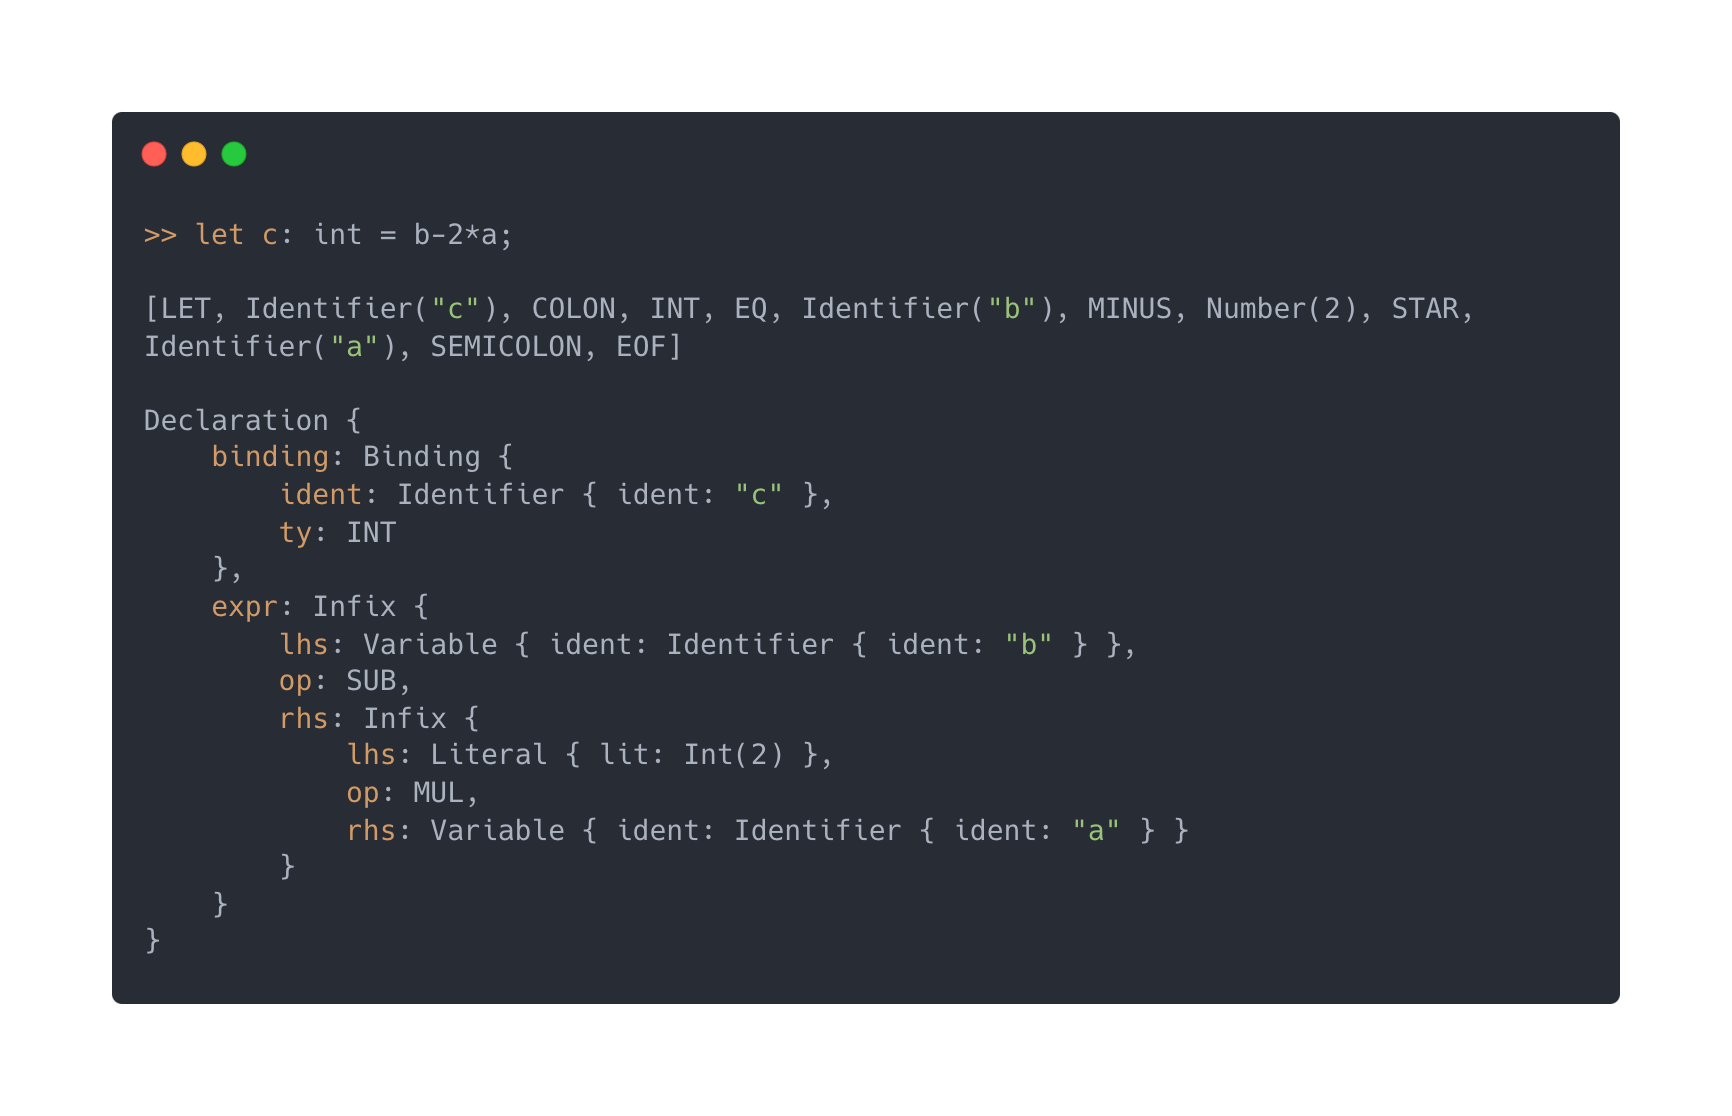
\includegraphics[width=12cm]{2. Unit Test.png}}
        & 
        The correct data types and expressions have been parsed.
        \\
    \hline
        \raisebox{-\totalheight}{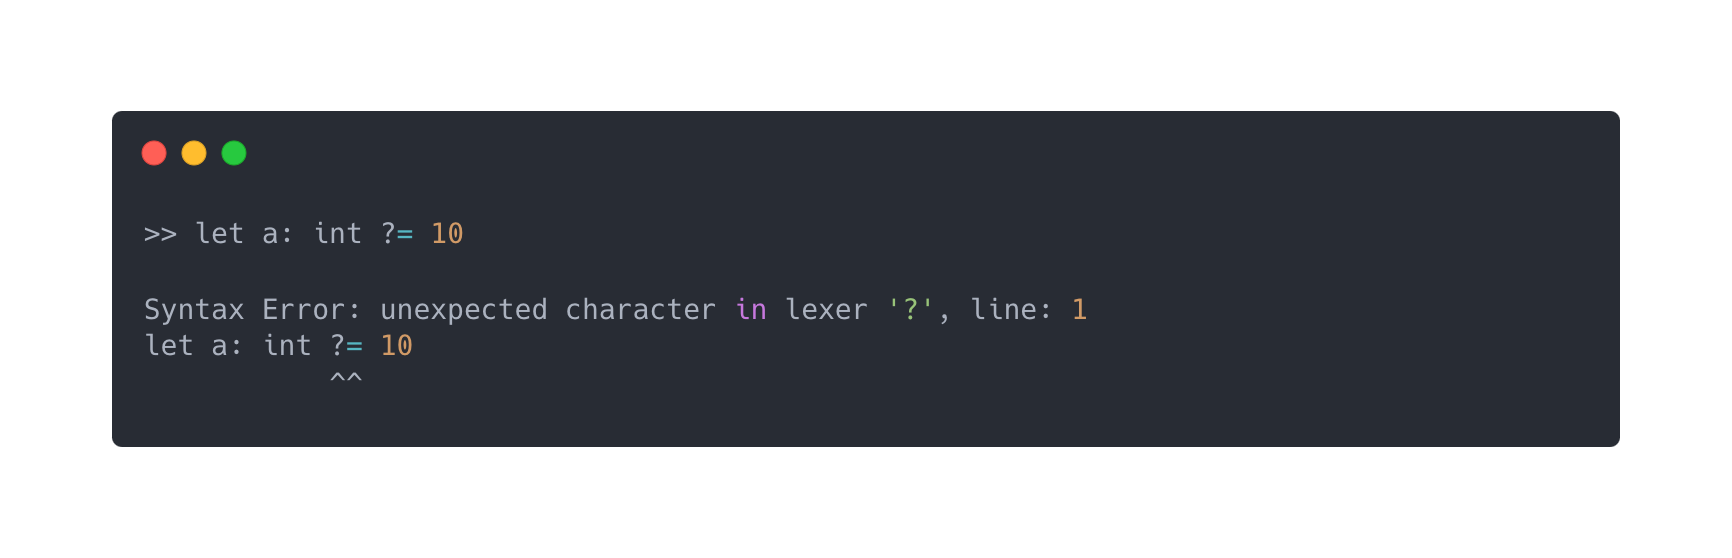
\includegraphics[width=12cm]{3. Unit Test.png}}
        & 
        A Syntax Error has been thrown successfully pointing to the location of the unexpected character in the source code
        \\
    \hline
        \raisebox{-\totalheight}{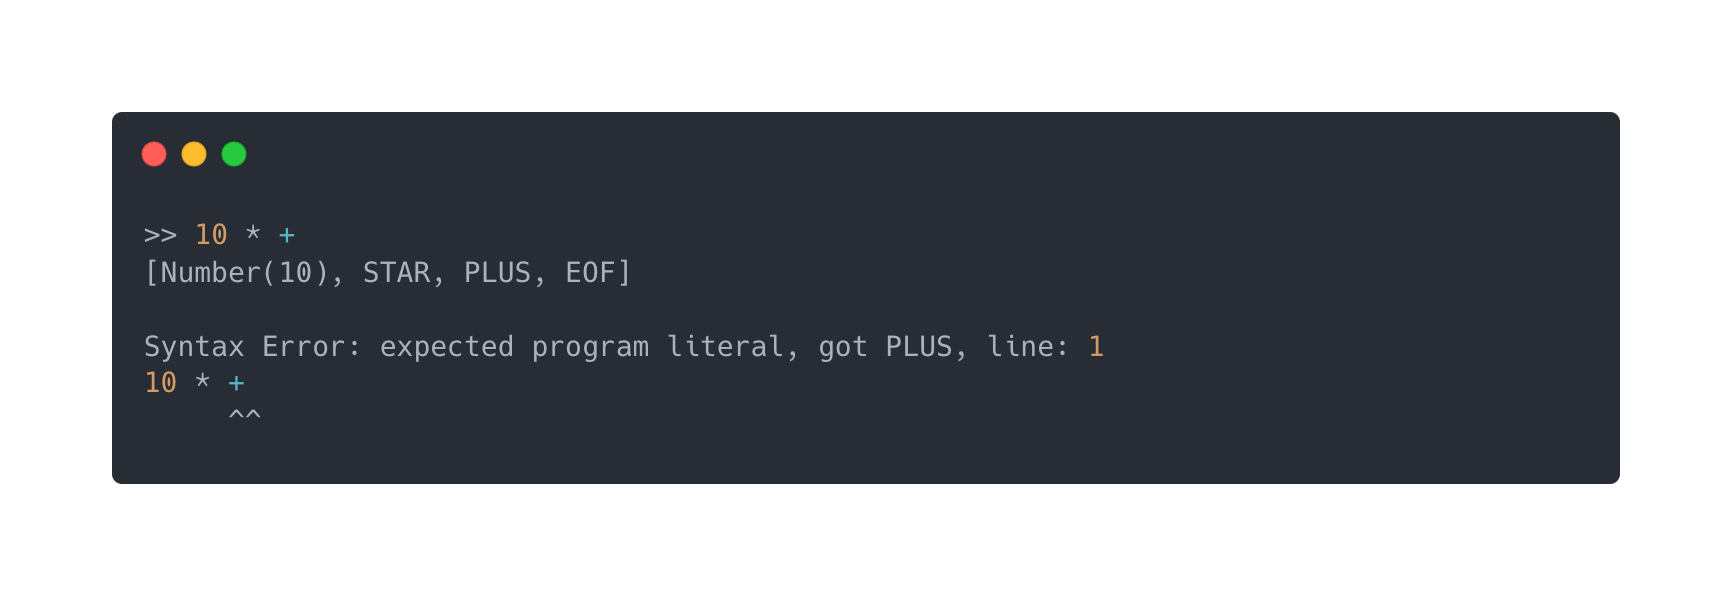
\includegraphics[width=12cm]{4. Unit Test.png}}
        & 
        A Syntax Error was successfully thrown and the program refused to compile.
        \\
    \hline
        \raisebox{-\totalheight}{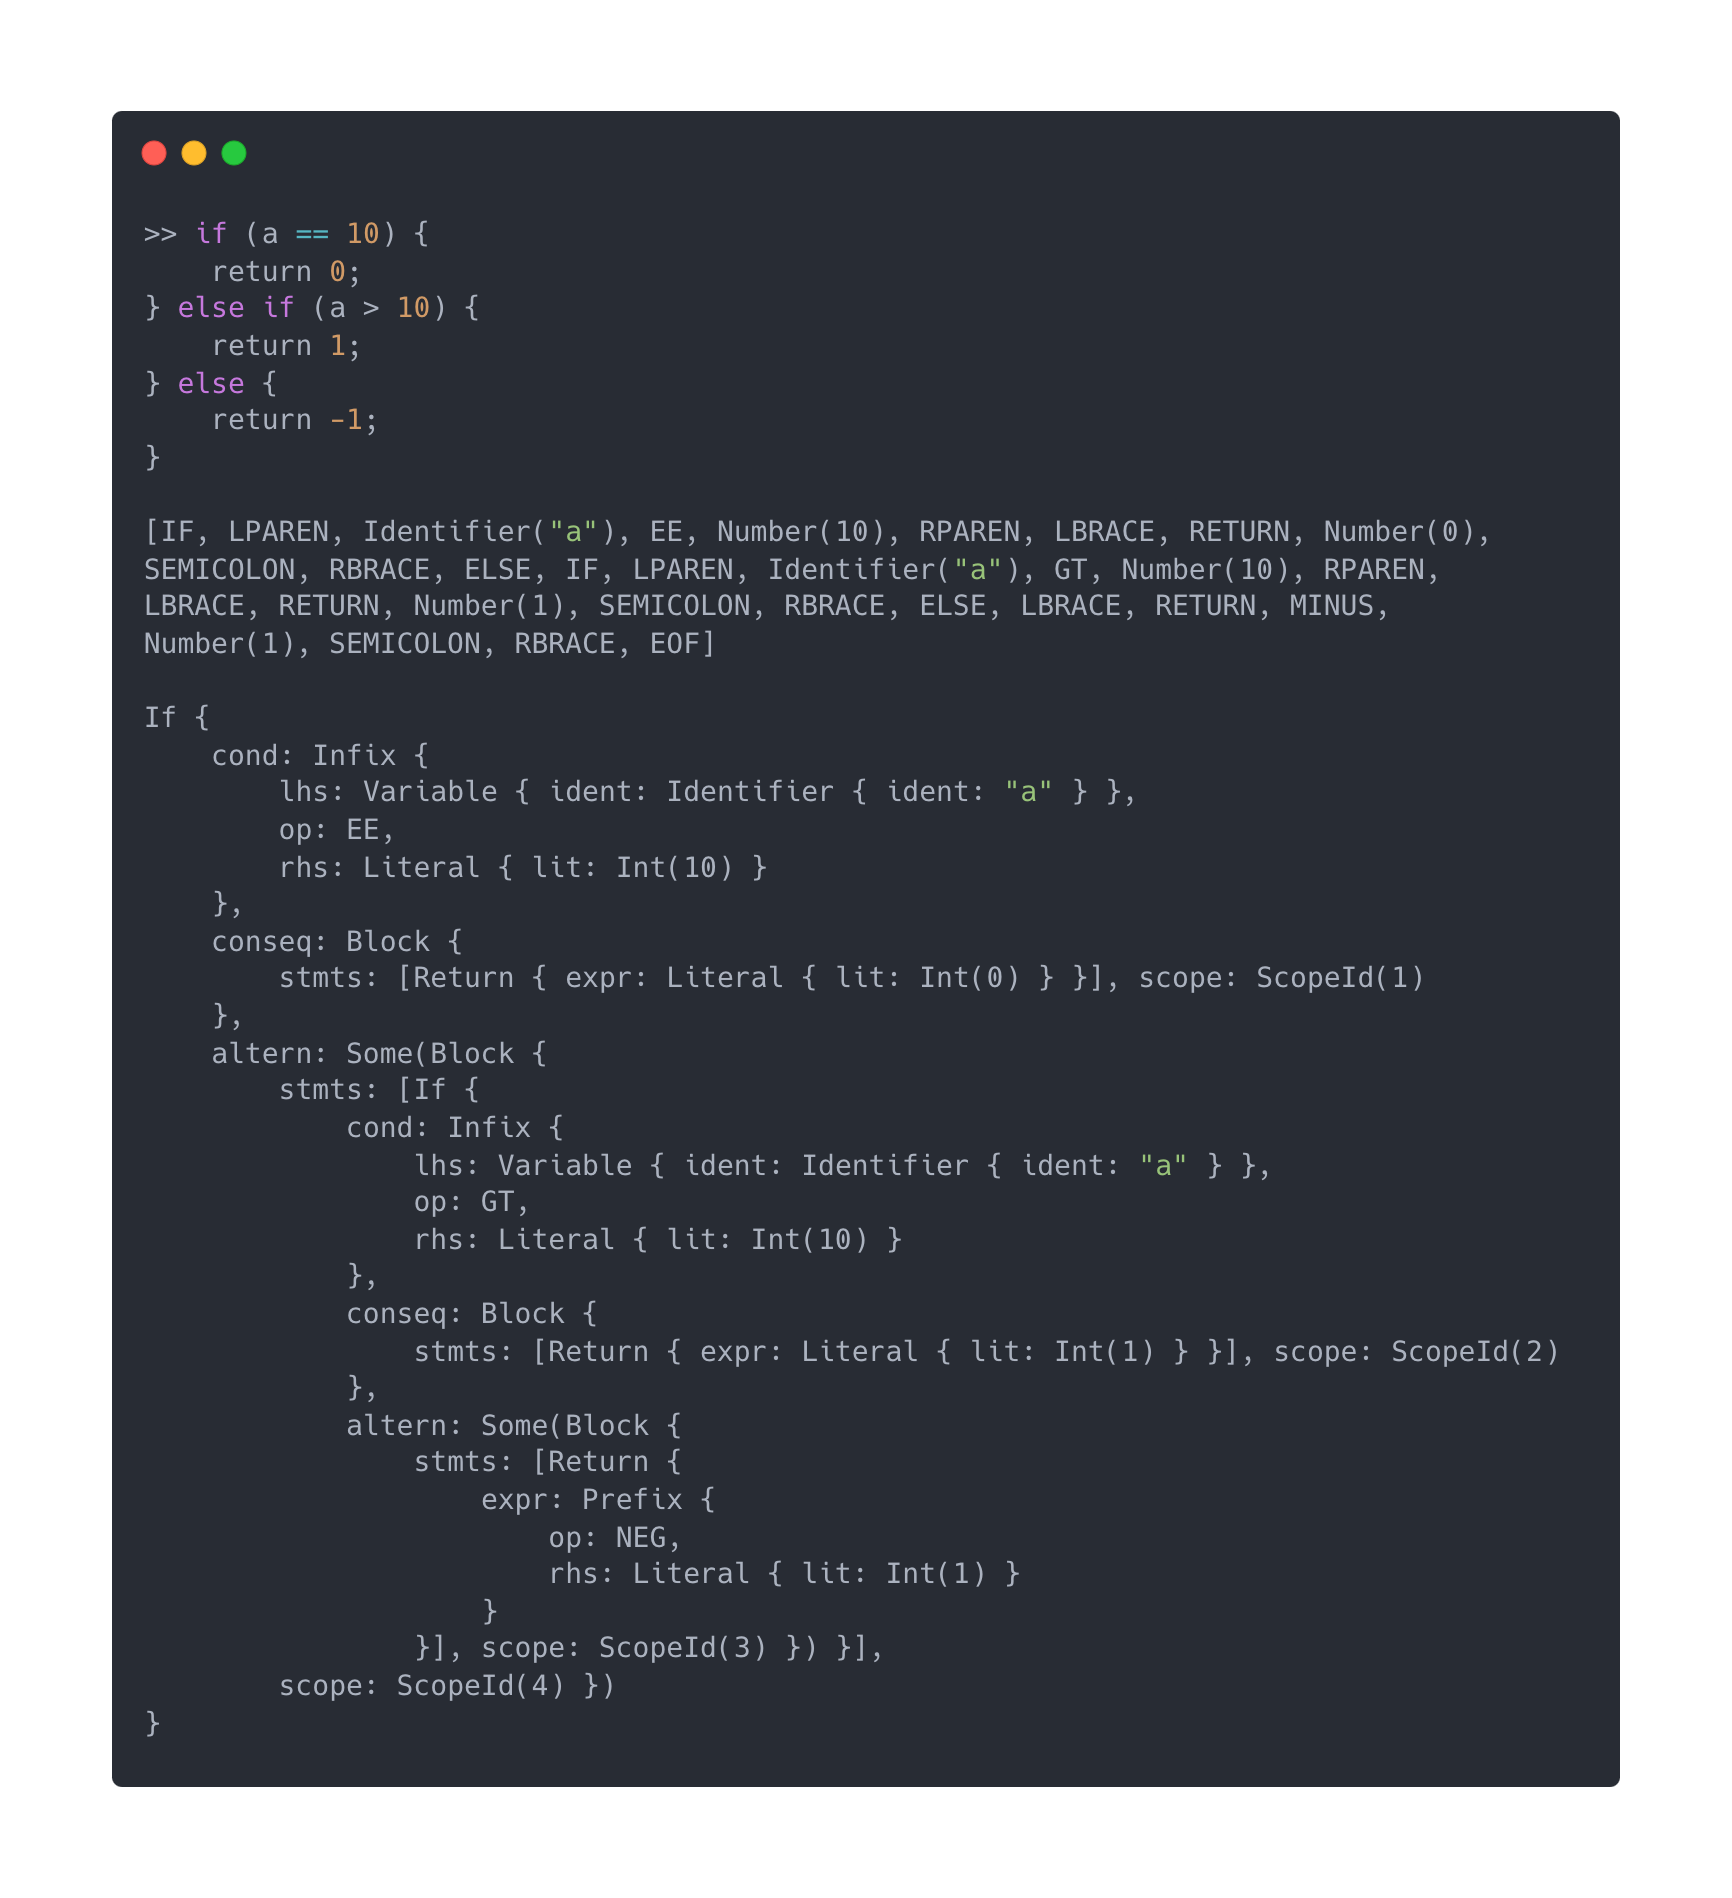
\includegraphics[width=12cm]{5. Unit Test.png}}
        & 
        The else-if clause was parsed as a seperate IF node inside the 'alternative' stmts attribute of the primary if node. Furthermore, each block was successfully assigned its own unique scope identifier and the prefix '-1' was parsed correctly.
        \\
    \hline
        \raisebox{-\totalheight}{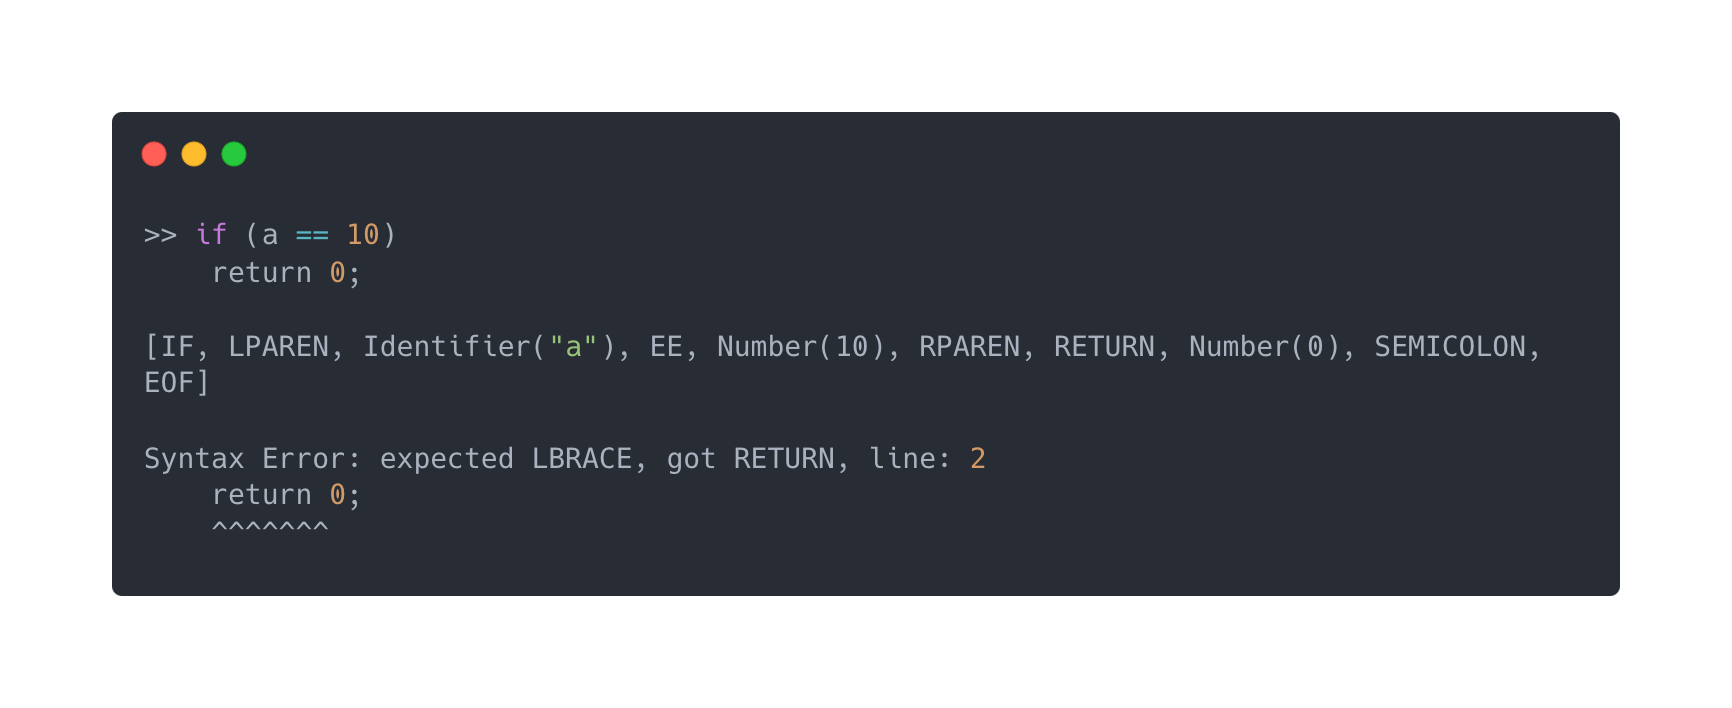
\includegraphics[width=12cm]{6. Unit Test.png}}
        & 
        When parsing the if statement, the parser expects a '\{' token, however instead, it encounters a 'return' keyword - it successfully halts compilation and throws an error as expected. 
        \\
    \hline
        \raisebox{-\totalheight}{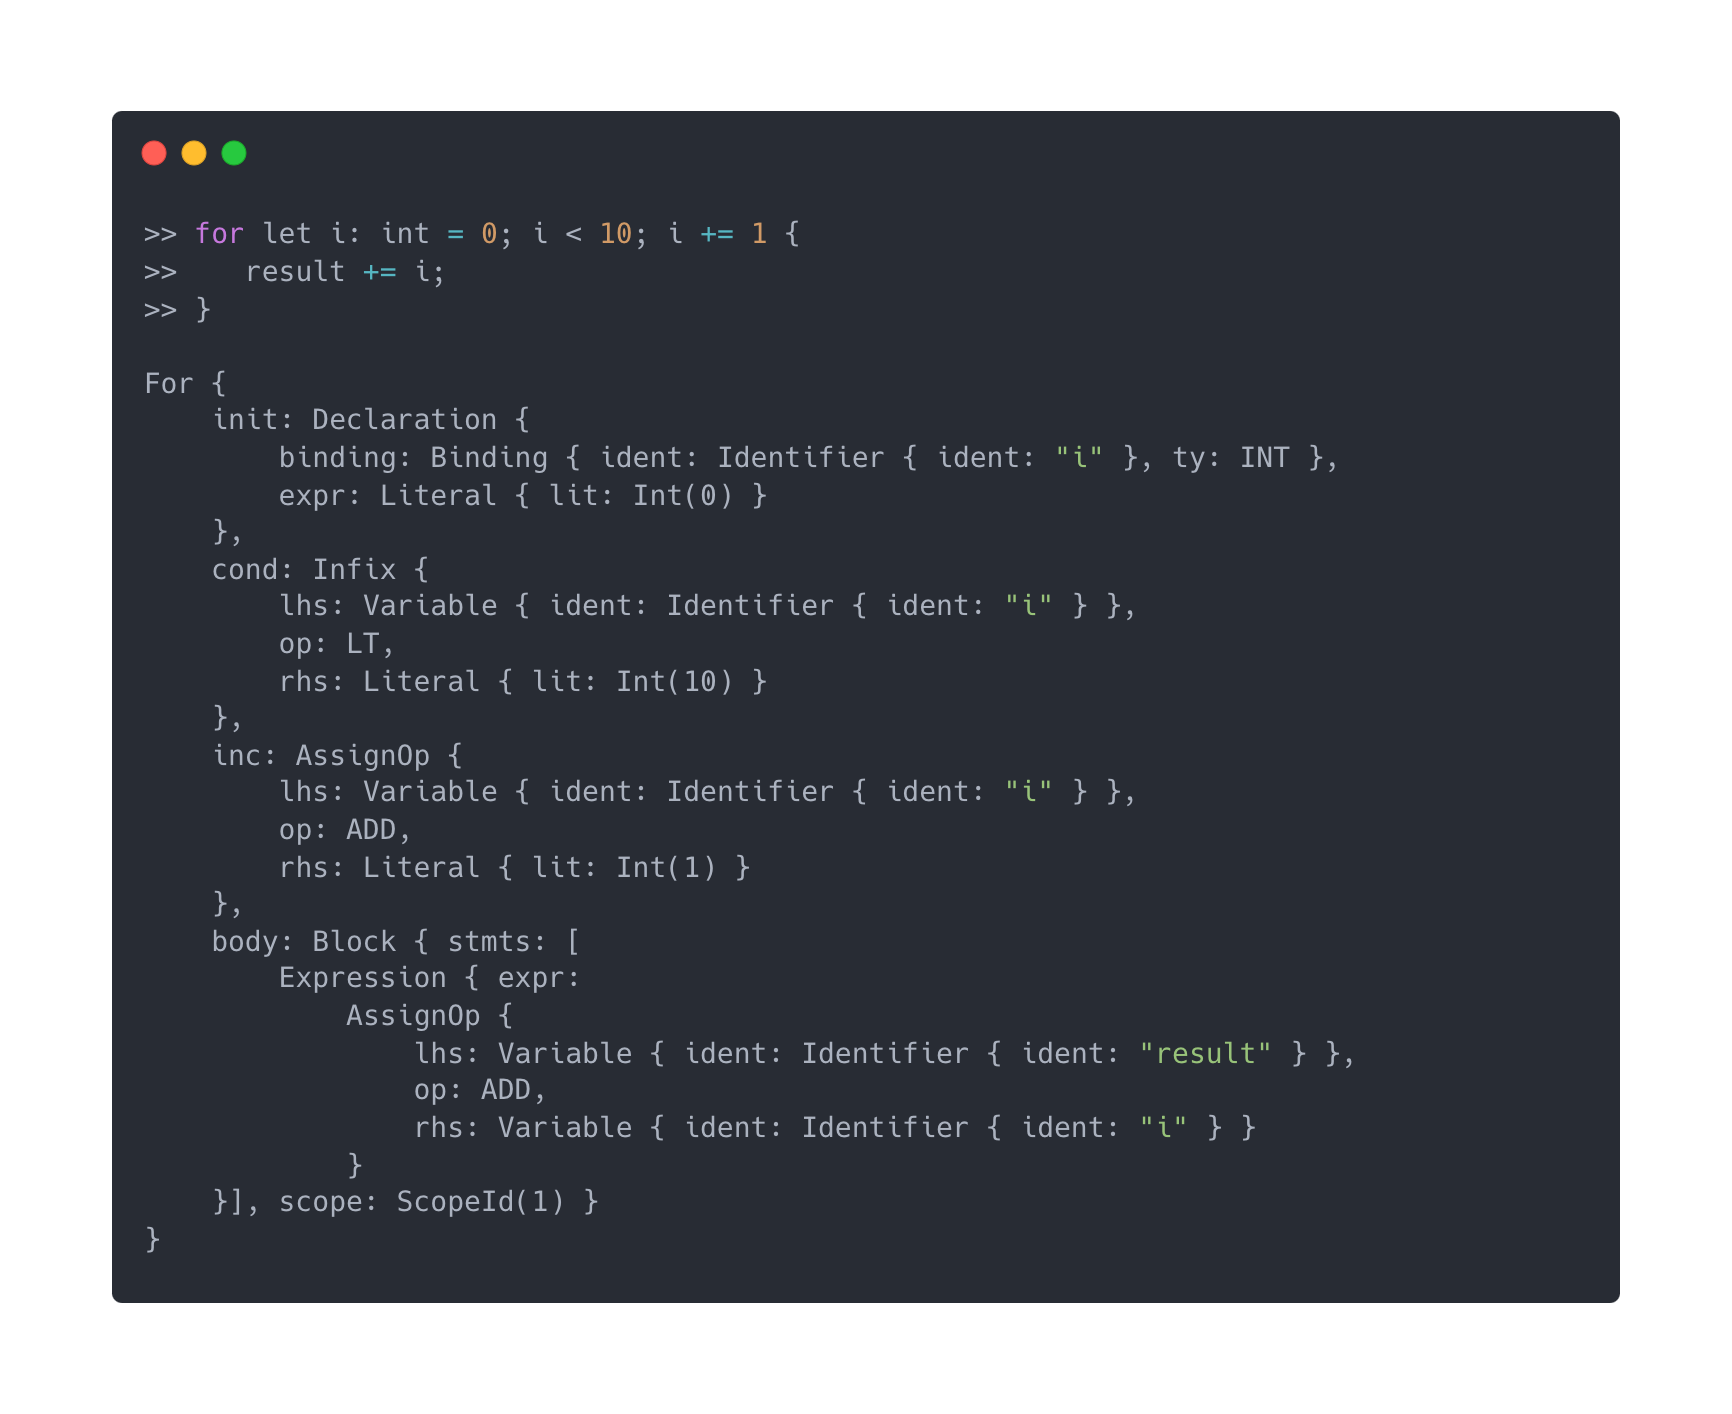
\includegraphics[width=12cm]{8. Unit Test.png}}
        & 
        The initialise, condition and increment fields are successfully parsed in the for loop, and the '+=' assign op is successfully identified as a 'plus' operation. 
        \\
    \hline
        \raisebox{-\totalheight}{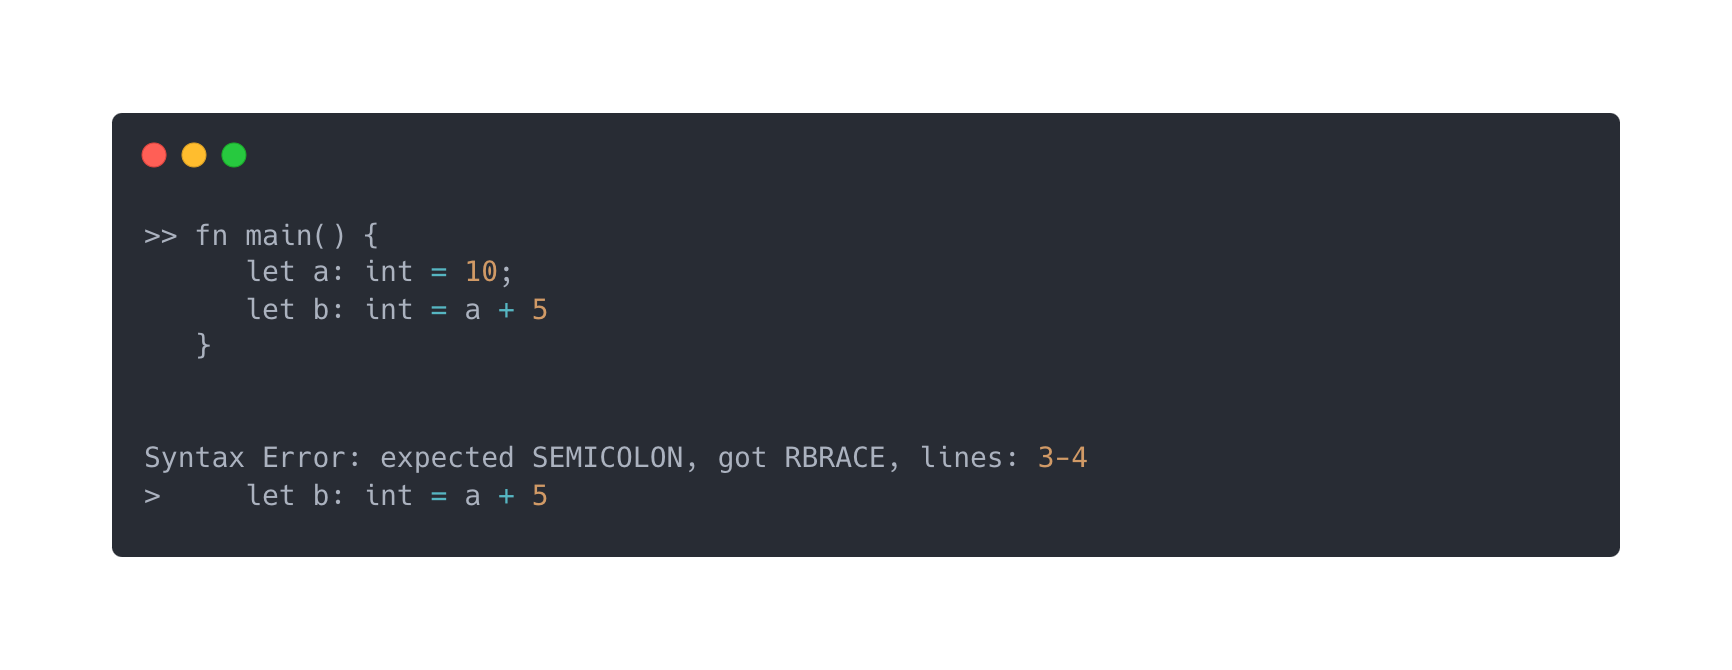
\includegraphics[width=12cm]{14. Unit Test.png}}
        & 
        The compiler notices that line 3 isn't terminated by a semicolon and throws an error, pointing out the location of the syntax error and halting compilation. 
        \\
    \hline
\end{longtable}

\subsubsection{Semantic Analysis}

The second part of the compiler that warrants further testing is the sentiment analysis. Once a valid program is successfully parsed, the produced abstract syntax tree is checked for further errors. For instance, referencing a variable which has not yet been declared, and validating the data types of expressions and assignments.  

\begin{longtable}{|p{12cm}|p{4cm}|} 
    \hline
        Program & Result \\ 
    \hline
        \raisebox{-\totalheight}{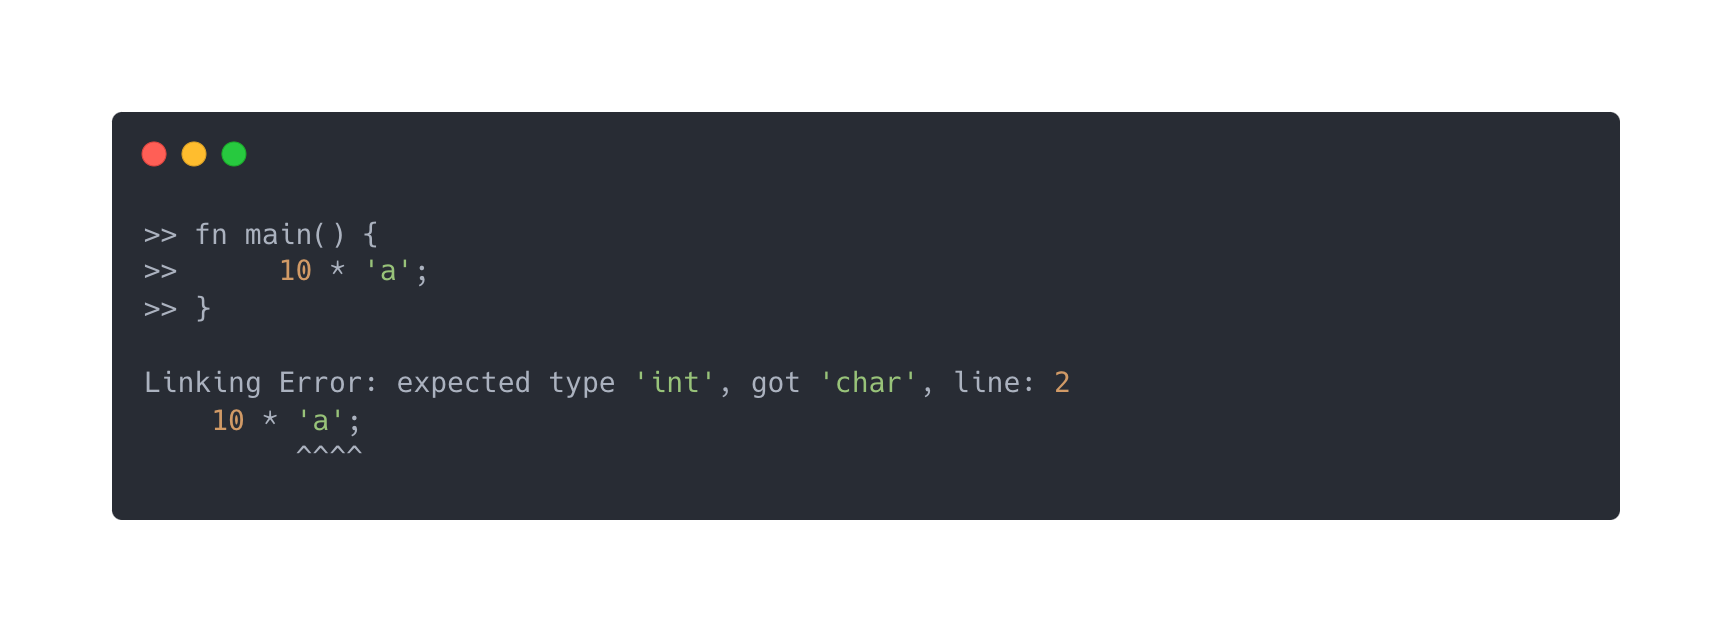
\includegraphics[width=12cm]{7. Unit Test.png}}
        & 
        The program successfully throws an error when it notices a type error, attempting to multiply an integer and character. 
        \\
    \hline
        \raisebox{-\totalheight}{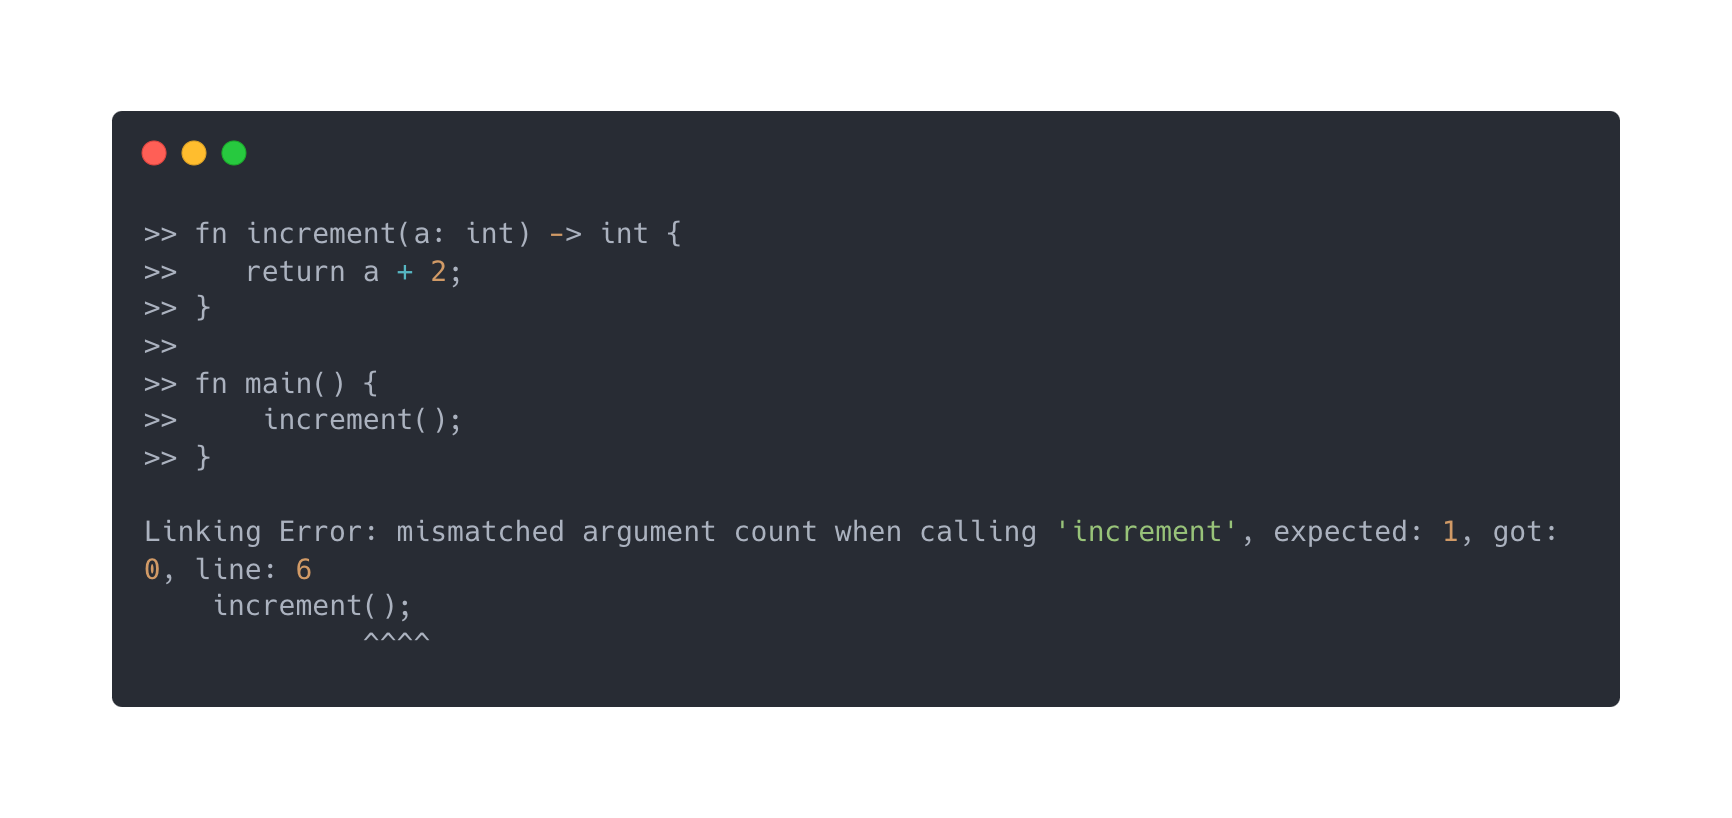
\includegraphics[width=12cm]{9. Unit Test.png}}
        & 
        The program successfully throws an error when attempting to call a function with the incorrect number of arguments.
        \\
    \hline
        \raisebox{-\totalheight}{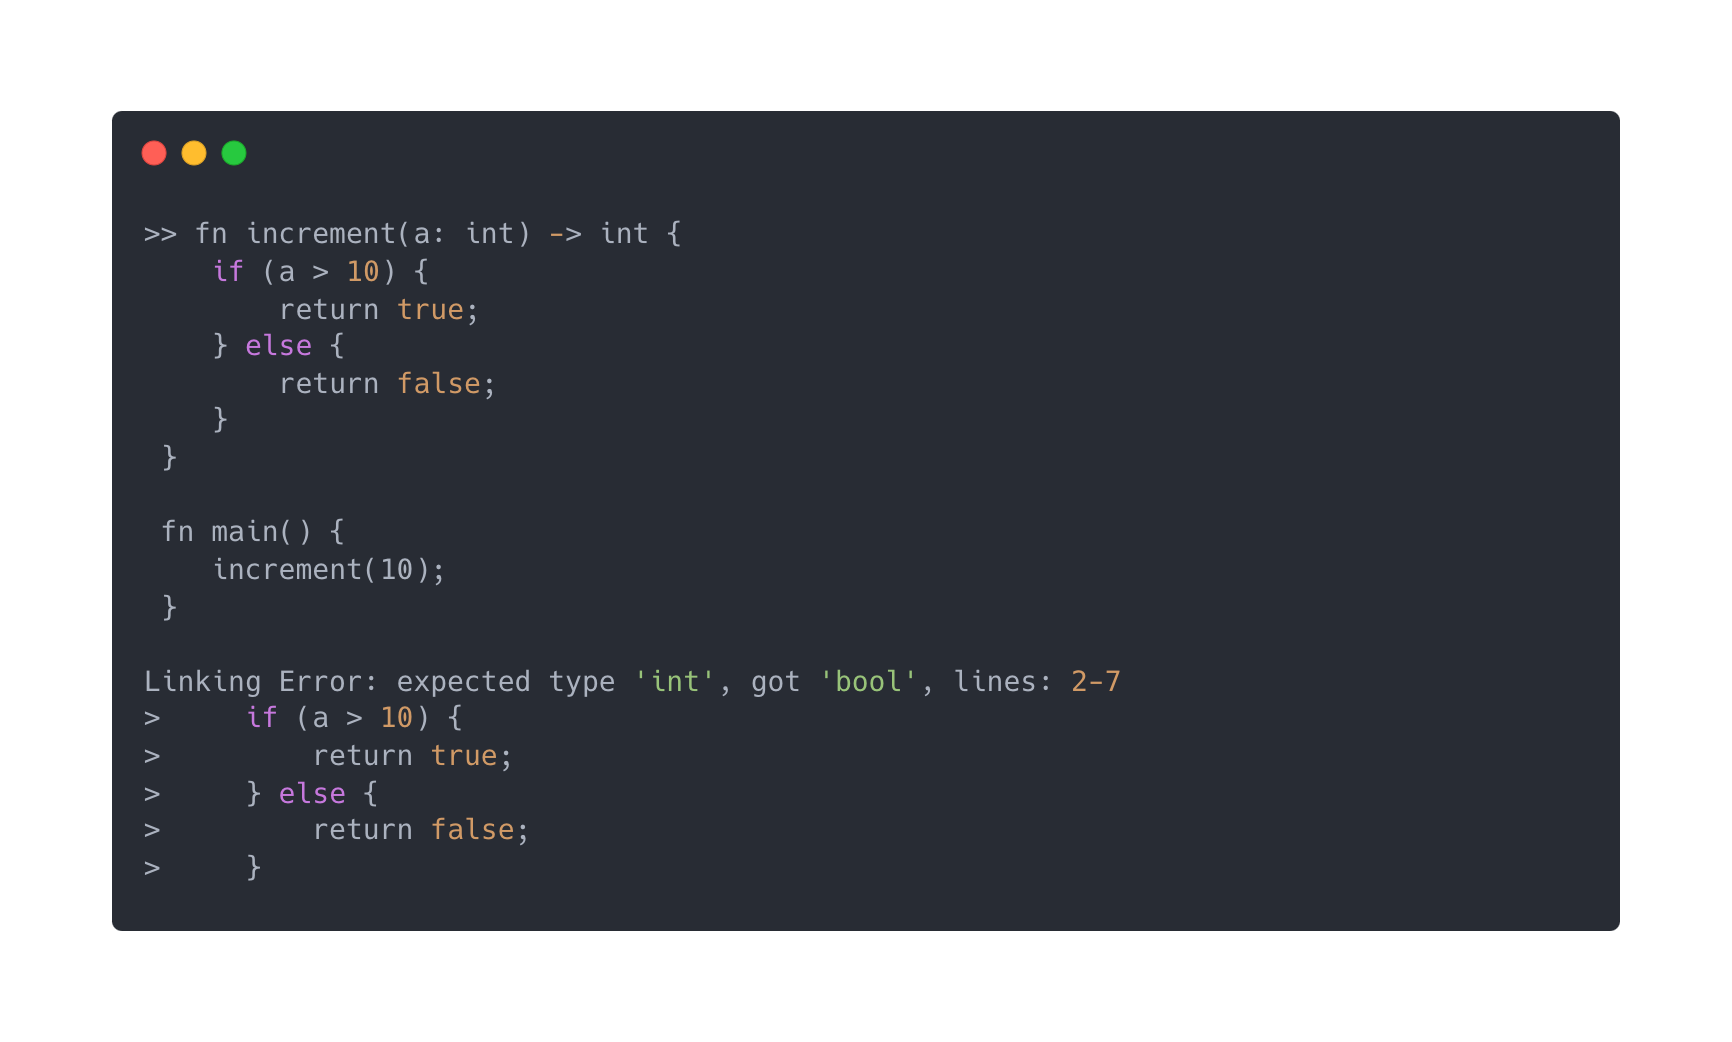
\includegraphics[width=12cm]{10. Unit Test.png}}
        & 
        The program notes that the function 'increment' is attempting to return an incorrect type. The compiler successfully notices that the 'return' expression occupies multiple lines and modifies the format of the error message accordingly.
        \\
    \hline
        \raisebox{-\totalheight}{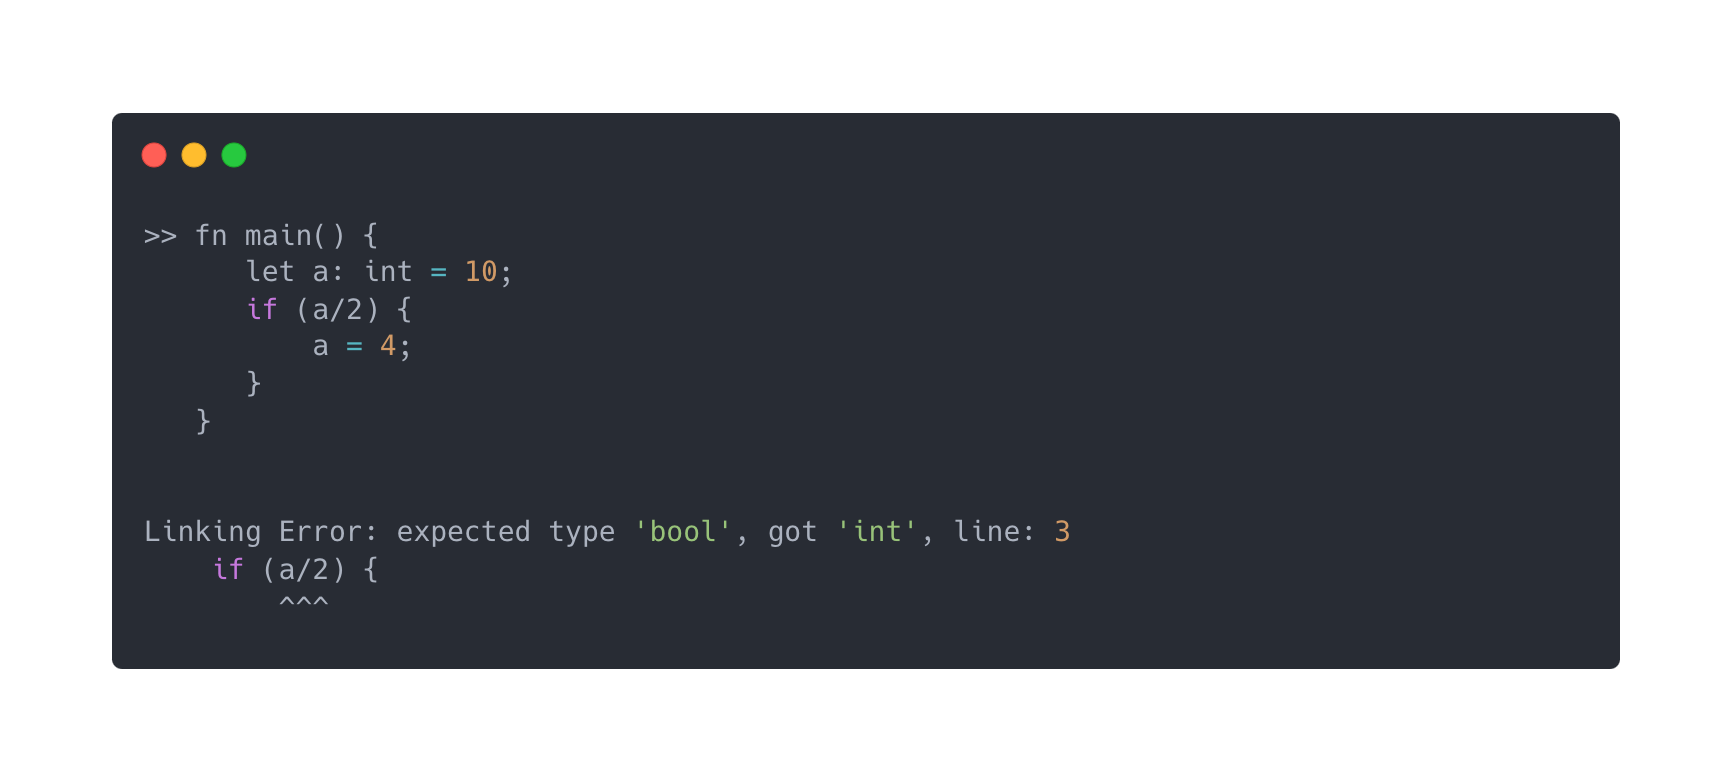
\includegraphics[width=12cm]{11. Unit Test.png}}
        & 
        The program throws an exception noting that the condition of the if-node will not evaluate to a boolean when executed. 
        \\
    \hline
        \raisebox{-\totalheight}{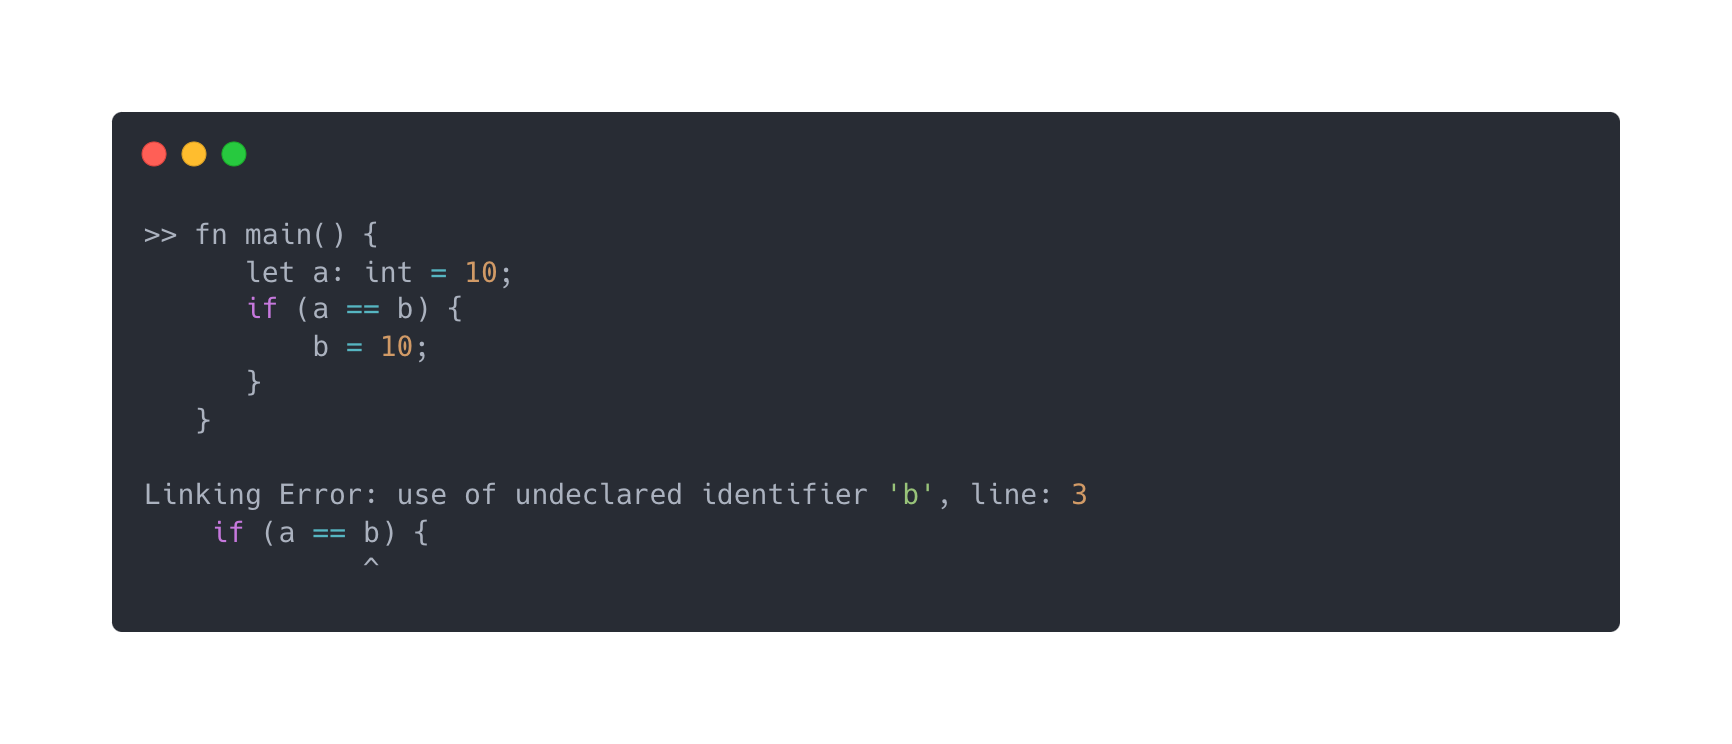
\includegraphics[width=12cm]{12. Unit Test.png}}
        & 
        The program throws an error and halts compilation when attempting to reference a variable that has not yet been declared.
        \\
    \hline
        \raisebox{-\totalheight}{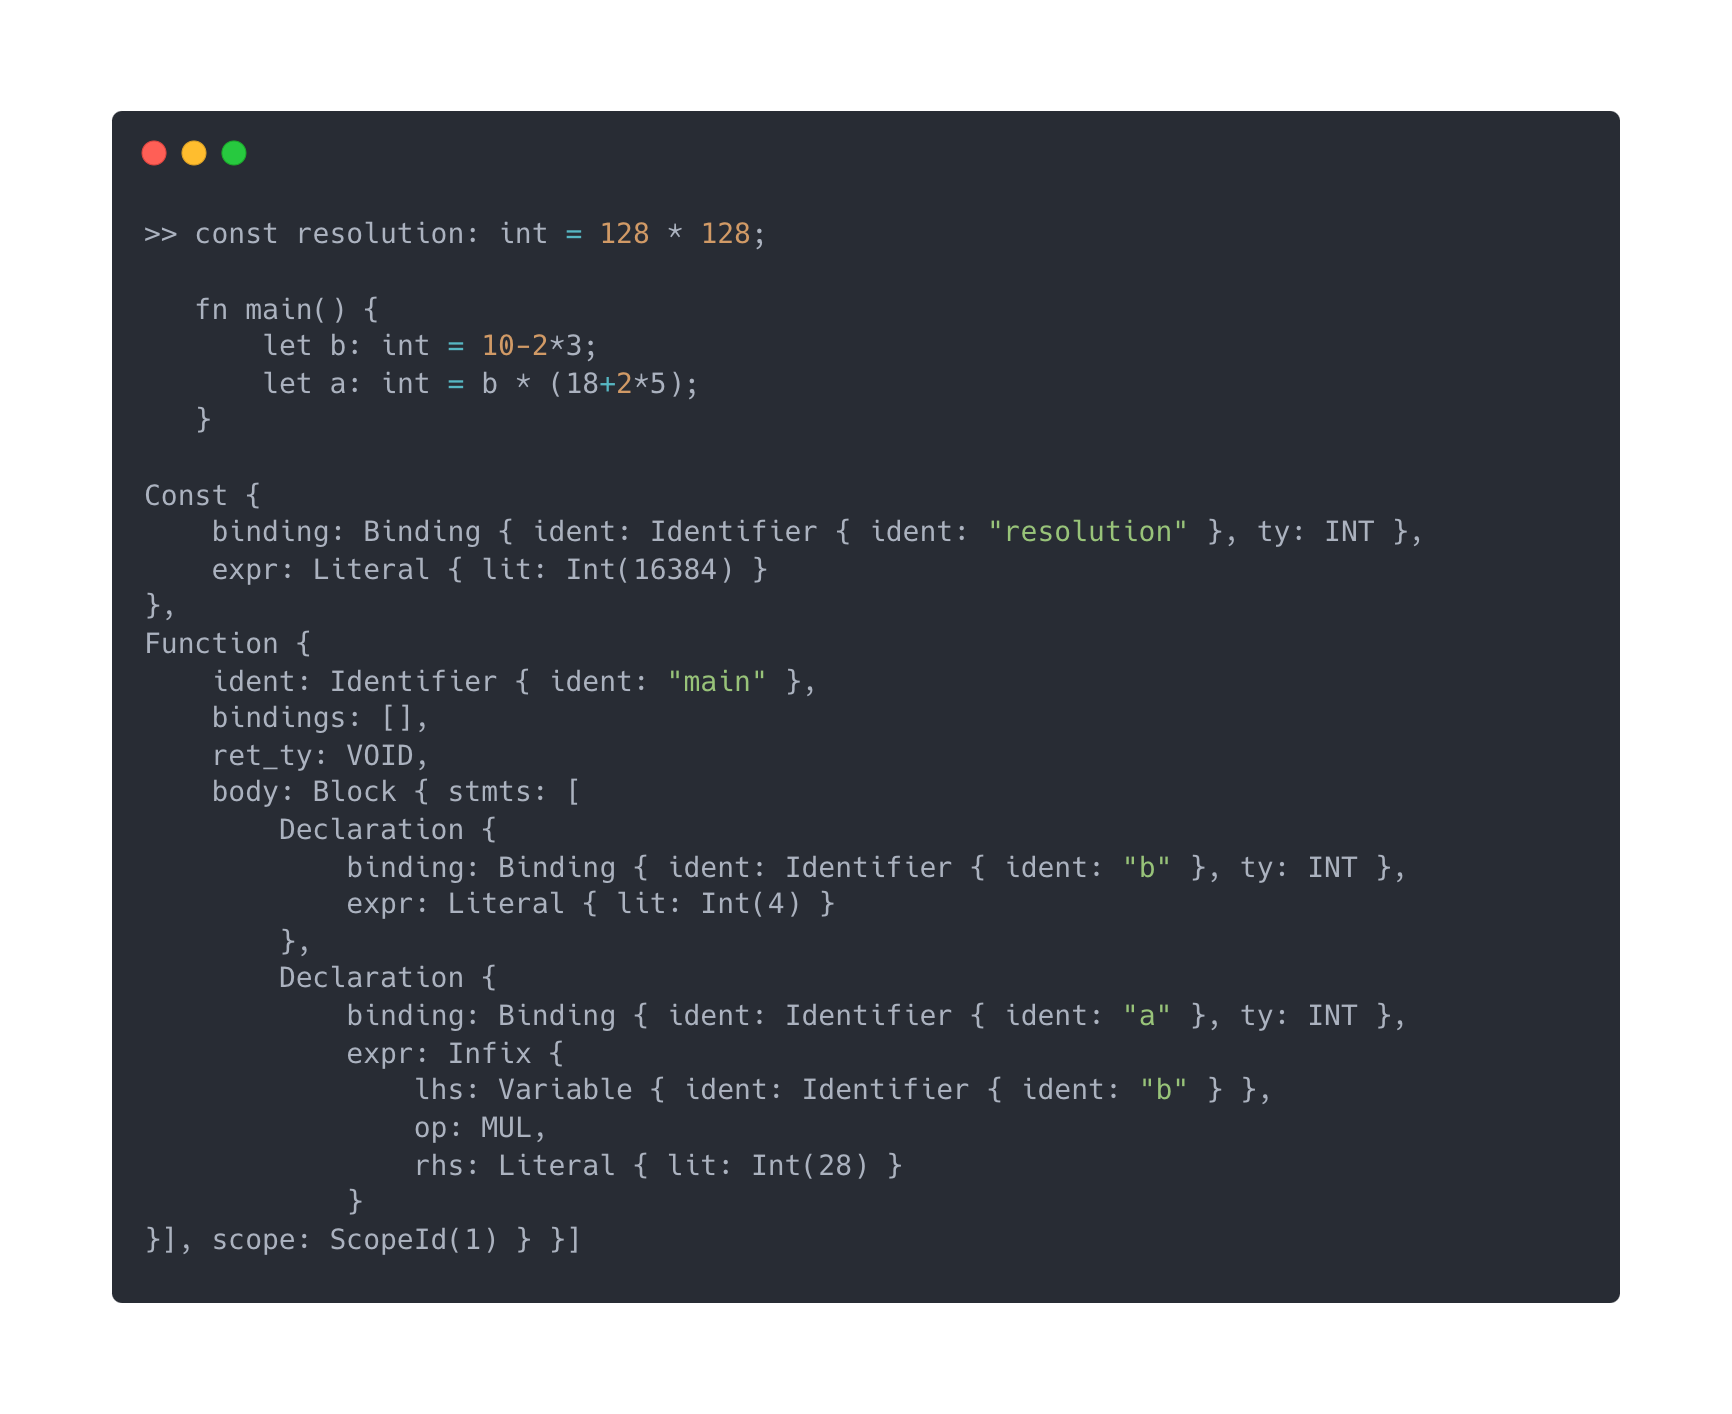
\includegraphics[width=12cm]{13. Unit Test.png}}
        & 
        This program demonstrates the process of constant folding in the compiler. The compiler successfully noticed that the expressions '128*128', '10 + 3*2', and '10+2*5' could be evaluated to integers, and replaced the entire expression with a single node containing its result. 
        \\
    \hline
\end{longtable}